\documentclass{article}

\usepackage{tikz}
\usetikzlibrary{automata, positioning}
\begin{document}
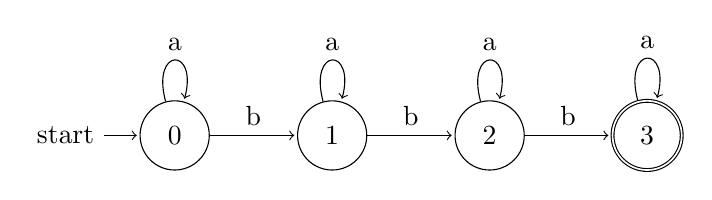
\begin{tikzpicture}[shorten >= 1pt, node distance = 2cm, on grid, auto]
  \node[state, initial] (0) {0};
  \node[state] (1) [right=of 0] {1};
  \node[state] (2) [right=of 1] {2};
  \node[state, accepting] (3) [right=of 2] {3};
  \path[->]
    (0) edge [loop above] node {a} (0)
        edge node {b} (1)
    (1) edge [loop above] node {a} (1)
        edge node {b} (2)
    (2) edge [loop above] node {a} (2)
        edge node {b} (3)
    (3) edge [loop above] node {a} (3);
\end{tikzpicture}
\end{document}
